\chapter{基于缓冲区分析的直播码率自适应算法}

很多现有的实时流媒体系统都是建立在UDP协议之上,相比于TCP协议而言,在带宽较低以及丢包率较高的网络中,UDP是一个更好的选择。在这样的网络状况下,TCP协议的实用性很弱,因为它的重传机制以及拥塞控制导致低吞吐量,带来难以接受的传输延迟。而UDP带来的实时性效果显著强于TCP,因为传输的数据包大小更小,并且不确保数据的完整接受。

然而,正因为UDP的不可靠的端对端传输,我们需要在更高层的协议之上进行大量特殊的处理,实现对传输过程进行控制以及对传输数据进行校验。而在另一方面,网络状况已经得到了持续快速的改善,使用TCP传输流媒体数据的可行性大大提高。因此,基于TCP的视频流媒体越来越成为关注的热点。渐进式HTTP视频流正广泛地应用在视频点播技术,并且通过HTTP Live Streaming(HLS)协议[1]扩展到视频直播领域。Real Time Streaming Protocol(RTSP)[2]以及Real Time Streaming Protocol(RTMP)[3]是两种业界广泛应用的,能够实现低延迟传输以及连接端进行消息交互的流媒体协议。这些基于TCP的技术很容易使用,并且在稳定的网络状况下具有良好的效果。然而,对于不稳定的移动网络,TCP吞吐量的变化仍然需要有效的应对,从而实现更好的流媒体用户体验。

在大多数的相关研究在两个层面处理TCP吞吐量的变化:传输层以及应用层。在传输层中,主要有两类方案。一类是通过修改TCP协议的重传机制和拥塞控制机制来降低吞吐量的波动[4][5],另一类是TCP传输层的信息建模来实现准确估计吞吐量从而选择最佳的视频编码参数。然而这一些方法难以具体实现,并且不能被应用在现有的基于TCP的应用层协议中。在应用层方面,研究主要集中在Dynamic Adaptive Streaming over HTTP(DASH)[6],它提供了客户端动态切换码率的机制来实现连续而平滑的视频点播服务。基于DASH的方案也同样被应用在HLS中实现自适应的直播视频流。然而DASH的自适应机制针对接收端,而不是内容提供方,因此不能应用在用户生成内容(UGC)的直播系统中。

在这篇论文中,我们提出一种通用的针对应用层的自适应码率控制方法来适应TCP吞吐量的变化,我们使用多缓冲模型来分析传输过程,并采用缓冲区的状态来评估网络状况。通过在这个模型获取到的信息,我们提出一种基于PID的自适应码率控制算法,能够灵敏地调节视频码率来匹配当前的网络吞吐量,从而在保证流畅播放的情况下提供最高能达到的视频质量。我们还对调节过程进行优化,使其尽可能稳定和准确。我们基于RTMP协议实现了手机视频直播系统,并采用了这种方法。我们在变化的网络状况下,实现了相对流畅的视频播放,并取得了高带宽利用率。
这篇论文剩下的部分主要包含以下内容:第二部分是传输架构的概述,第三部分描述了多缓冲模型,第四部分详细介绍了基于PID的自适应码率控制算法,第五部分展示了在不同条件下的实验结果,第六部分进行了总结。

\section{视频直播系统概述}

在有些视频直播系统中,视频内容由服务器或者与服务器通过局域网连接的设备生成。在这种情形下,视频直播和视频点播具有很多共同点。在直播中服务器将动态生成的视频数据发送给客户端,和点播最主要的区别在于传输速率不能超过视频数据生成速率,因此当所有生成的数据都传输之后,客户端需要等待下一个数据片段就绪\supercite{Thang2014}。而在如今十分火热的用户生成内容(UGC)直播模式下,服务器本身不充当初始的内容产生方,在其他设备上持续生成的视频内容经过不确定且不可忽略的延迟传输到中转服务器。目前已经非常普及的智能手机成为了理想的内容产生方和接收方。图\ref{fig:07}展示了通用的手机视频直播系统的主要模块。集成了高效视频编码器的智能手机,将实时视频数据传输到接收服务器,在此同时,原始视频流被转码成多路具有不同码率的视频流。客户端可以通过当前网络环境选择最合适的码率,从服务器获取视频数据。

\begin{figure}[h]
	\centering
	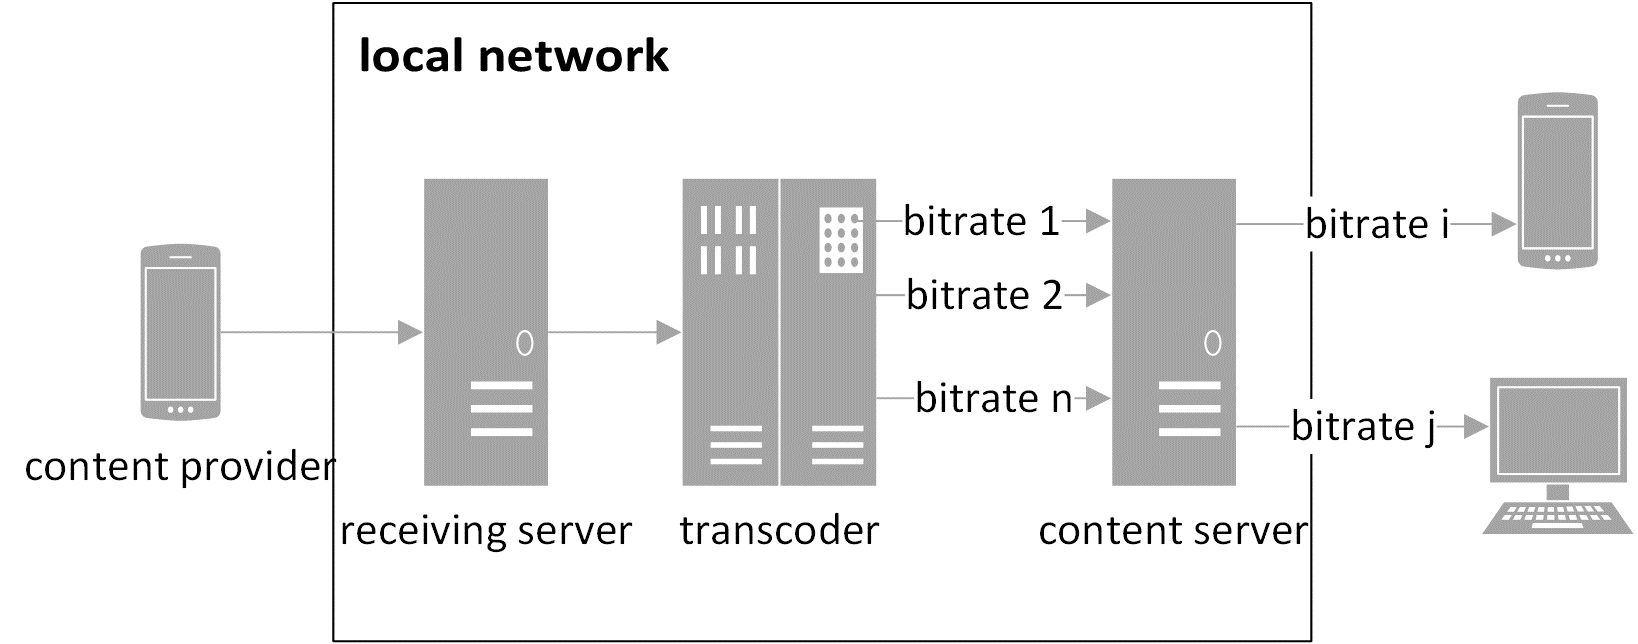
\includegraphics[width = 0.9\linewidth]{clip/07.png}
	\caption{通用的手机直播系统模型\label{fig:07}}
\end{figure}

为了提供高质量的直播视频流,内容产生方需要传输尽可能高码率的视频,这可能导致每个数据段传输时间过长,造成接收端的播放中断。而内容产生方在变化的网络状况下尽可能利用网络吞吐量传输高质量视频的同时保证接收端的流畅播放,是一个挑战。与此同时,延迟需要控制在一个可以接收的范围。我们在内容产生方设计了一个上传码率自适应控制器,这种方案能够应用于UGC的视频直播。

简单起见,我们假设服务器具有快速的内部操作,同时接收端通过稳定高效地网络与服务器进行连接,这意味着服务器和接收端的视频流与内容产生方和服务器的视频流保持同步。这个假设对我们的研究重点没有影响。我们将传输架构简化成如图\ref{fig:08}所示。内容产生方的编码器将输入视频压缩之后传递给基于TCP的应用层协议。经过各层协议的封装,数据被传递到网络进行实际传输。在接收端经过一个逆向过程之后,数据输入到解码器进行解码,然后在播放器中进行渲染。与此同时,在发送方的自适应控制器每隔特定的周期对传输信息进行检查,并采用后文将介绍的特定的策略对编码器参数进行调整。

\begin{figure}[h]
	\centering
	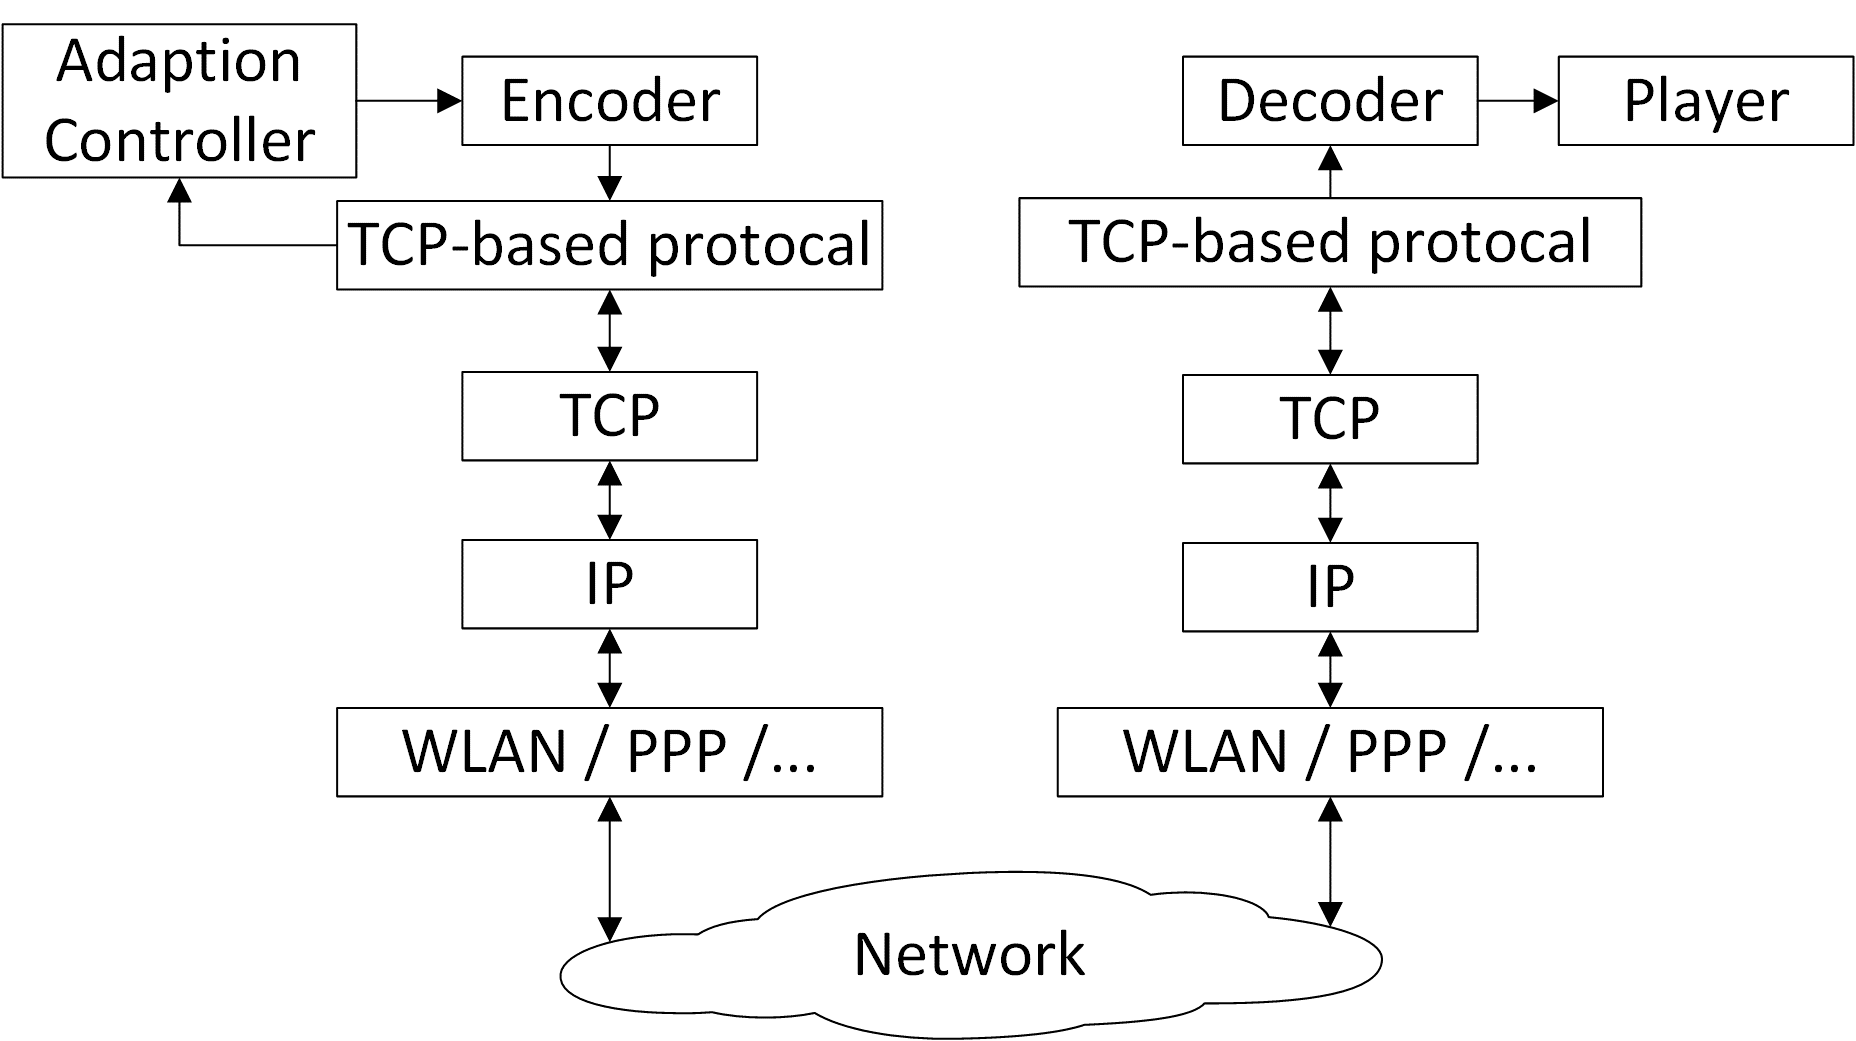
\includegraphics[width = 0.9\linewidth]{clip/08.png}
	\caption{简化的直播系统传输架构\label{fig:08}}
\end{figure}

\section{直播中的多缓冲区模型}

\subsection{TCP缓冲区}

几乎所有的现代操作系统都集成了TCP协议,它是一种网络传输层协议。在传输过程当中,TCP协议采用了一种滑动窗口机制来保证可靠性,同时控制流量。为了实现滑动窗口机制,采用了TCP发送缓冲区(TSB)来缓存将要发送的数据同时维护滑动窗口,以及TCP接收缓冲区(TRB)来缓存接收成功但未被上层协议获取的数据。TSB中的数据收在到接收确认之后才会被移除,而TRB中的数据在被上层协议获取之后才会被移除。只有当TRB中存在足够空间的时候,网络传输才会进行。

\subsection{应用层发送缓冲区}

根据TCP的传输过程,只有当TSB中存在足够空间的时候,上层协议才能够将数据放入TSB。否则,上层协议的进程将会被阻塞,等待TSB中缓存的数据被移除。我们将第$i$次阻塞时间表示为$\varDelta t(i)$,将传输视频的帧率表示成$f$,并假设每一个数据段内的视频帧数为$n$。如果对于所有的$i$,都满足$\varDelta t(i) \le n/f$,那么这是较为理想的情况,因为不存在发送数据的积累。否则,在产生阻塞的时候需要采用应用层发送缓冲区(ASB)来缓存持续产生的视频数据。当TSB中产生足够的空间的时候,ASB队列头部的数据将会被移除进行发送。我们定义ASB的长度为其中数据段的数量,在大多数情况下我们期望它是一个较小的值。在通常情况下,存在ASB的最大长度。如果ASB达到了最大长度,后面到来的数据段将会被丢失。ASB长度上限的设置是一种通用的限制延迟的方法。

\subsection{播放缓冲区}

当ASB的长度增长的时候,发送端将在大于$n/f$的间隔时间收到两个连续的数据段。在这种情况下,为了保持连续的播放,几乎所有播放器都会设置一个播放缓冲区(PB),它从TRB中获取数据,并按照固定的速率将数据解码并显示。当PB的长度的为0时,视频停止播放直到PB的长度增长到一个固定值。我们称这个值为初始值,并表示为$S_0$。在很多系统中,这种方法被证明十分有效,它弥补了短时间视频码率和网络带宽的不匹配,有效减少了视频中断的现象。通常情况下,$S_0$就是PB的最大长度,达到$S_0$的时候数据段在接收端将被丢弃。

图\ref{fig:20}展示了接收端的数据曲线。$G(t)$表示在时间$t$之前在内容产生方生成的数据段的数量,因此$G(t) = \mu t$,其中$\mu$是一个常量,表示数据段生成的速率。$A(t)$和$P(t)$表示在接收端接收到和播放的数据段的数量,图中有$S(t) = A(t) - P(t)$。第一个数据段在经过传输延迟$d_t$之后到达接收端,PB开始接收到数据。我们假设在时间$t_0$,第一次使得$S(t_0)=S_0$,开始进行播放。$t_0$可以看做播放延迟,我们表示成$d_p$。因此,存在$S(t) \le \mu (d_p - d_t)$。当$S(t)$减小到$0$,播放终止,直到$S(t)$重新增长到$S_0$。

\begin{figure}[t]
	\centering
	
\includegraphics[width = 0.8\linewidth]{clip/20.png}
	\caption{直播系统接收端数据关系\label{fig:20}}
\end{figure}

\subsection{多缓冲区模型分析}

如上文所讨论的,在传输架构中有四个缓冲区:TCP发送缓冲区、TCP接收缓冲区、应用层发送缓冲区、播放缓冲区,他们组成了多缓冲系统。在图\ref{fig:21}中,$G(t)$、$P(t)$以及$A(t)$与上一小节讨论的定义相同,$D(t)$表示在时间$t$之前进入TSB的数据段数量。我们使用$S_b(t)$表示在时间$t$存在于缓冲区$b$的数据段的数量。因此存在:
\begin{equation}
\label{eq:mm-1}
S_{ASB}(t)=G(t)-D(t),
\end{equation}

\begin{equation}
\label{eq:mm-2}
S_{TSB}(t)=D(t)-A(t),
\end{equation}

\begin{equation}
\label{eq:mm-3}
S_{TRB}(t)=A(t)-A(t)=0,
\end{equation}

\begin{equation}
\label{eq:mm-4}
S_{PB}(t) =A(t)-P(t),
\end{equation}

\begin{equation}
\label{eq:mm-5}
S_{ASB}(t)+S_{TSB}(t)+S_{TRB}(t)+S_{PB}(t)=G(t)-P(t).
\end{equation}


公式\ref{eq:mm-3}表示TRB的大小为0,因为在TRB中所有完整的数据段都会迅速被获取。当,即播放进行的时候,存在$G(t)-P(t)=\phi$,$\phi$是一个常量,反映了播放延迟。因此我们可以得到
\begin{equation}
\label{eq:mm-6}
S_{ASB}(t)+S_{PB}(t)=\phi-S_{TSB}(t).
\end{equation}
当$S_{ASB}(t)=0$,$S_{TSB}(t)$被$A(t)$所决定,它反映了网络状况。当$S_{ASB}(t)>0$时,意味着在发送数据到TSB时发生了阻塞,TSB一直处于充满状态,$S_{TSB}(t)$达到了上限,我们表示为$\alpha$。在这种情况下,存在
\begin{equation}
\label{eq:mm-7}
S_{ASB}(t)+S_{PB}(t)=\phi-\alpha=\delta.
\end{equation}
这表示着可以通过ASB的变化来控制和估计PB的变化。当$0 < S_{PB}(t) \le S_0$的时候,播放是连续的,可以通过保持$\delta - S_0 \le S_{ASB}(t) < \delta$进行实现,其中$\delta \ge S_0$。为了实现最小的延迟,$\delta$期望被设置为$S_0$。

\begin{figure}[t]
	\centering
	
\includegraphics[width = 0.8\linewidth]{clip/21.png}
	\caption{多缓冲区模型结构图\label{fig:21}}
\end{figure}

多缓冲系统的信息在应用层可以被很容易地获取,我们可以根据这些信息在内容产生方设计一个自适应控制器来执行自适应码率控制。


\section{码率自适应算法}

在这一部分,我们详细介绍自适应码率控制方法。我们希望自适应过程实现以下几个目标:(1)接收端能够连续播放;(2)传输和当前吞吐量匹配的最高视频质量;(3)尽可能低的延迟;(4)在快速波动的网络状况下灵敏地自适应;(5)方法具有通用性,能够容易地实现。对于目标(5),我们的方法建立在通用的基于TCP的模型上,并采用了应用层参数。对于目标(3)和(4),我们考虑了最小可调度单元(MSDU)。对于目标(1)和(2),我们提出了一种新的基于PID控制的方法,能够动态地将系统保持在理想状态。

\subsection{最小可调节单元}

我们定义MSDU为我们能够完整传输或丢弃的最小的单元。在我们所讨论的系统中,MSDU为数据段。数据段的小大可以在两个方面对系统产生影响:(1)传输延迟,数据段中的数据越多,第一个数据段完整到达接收端需要的时间就越长;(2)自适应的灵敏度,一次自适应调整只有在正在进行的传输过程结束之后才会起作用。因此我们期望数据段的大小能够最小。

在基于DASH的方案中,为了实现高度灵敏的切换,图像组(GOP)被设定为数据段[12]。一个GOP可以单独播放,包含了一个I帧以及多个P帧。当一个GOP被丢弃时,对其他的GOP没有影响。通常一个GOP的持续时间是1到5秒。

在我们的方法中,我们将MSDU设置为视频帧,这样可以讲传输延迟最小化,以及将自适应的灵敏度最大化。当一帧被丢弃时,我们需要丢弃其整个GOP中后续的P帧,这样不会带来解码的错误。

\subsection{状态变量选取}

使用PID进行码率自适应的关键在于选取一个能够反映传输状况的过程变量。基于TCP的直播系统在传输过程中有四个缓冲区,分别是应用层发送缓冲区(ASB)、TCP发送缓冲区(TSB)、TCP接收缓冲区(TRB)、播放缓冲区(PB)。这几个缓冲区的关系和意义如图\ref{fig:20}和\ref{fig:21}所示。其中对内容产生方最重要的信息是ASB内的数据长度,记为$S_{ASB}(t)$(在时刻$t$的值),它能够直接反映视频码率和吞吐量之间的匹配情况。当视频码率高于当前的吞吐量时,该缓冲区内的数据长度趋向于增大,否则保持相对稳定或者减小为0。理想状况下,它首先应该是一个大于0的值,以保证接收方播放不中断;其次它不应该太大,否则意味着发送码率太高。所以,我们选择$S_{ASB}(t)$作为系统的过程变量,而选择一个接近0的常量$\varepsilon$作为控制目标。

然而,如果网络吞吐量在一个小的范围频繁波动,将使得系统变量值不稳定而且相对随机,导致不必要的频繁的调整。为了消除这样的随机性,我们将过程变量的定义修改为$\overline{S_{ASB}(t)}$,它表示在时刻$t$之前的一个时间段$\tau$内$S_{ASB}(t)$的平均值。它可以表示为:
\begin{equation}
\label{eq:asb}
\overline{S_{ASB}(t)} = \dfrac{1}{\tau} \int_0^\tau {S_{ASB}(t)}\: .
\end{equation}

对于UGC直播应用来讲,由于发送的码流是实时生成的,所以调整码率时直接改变编码器参数以改变生成码率即可,不需要涉及码流截取等数据源端的操作。但是,质量等级的概念仍然需要,它在这里变成了改变码率的单位。控制模型可以直接采用原始PID中的做法,用过程变量和$\varepsilon$的差值来计算比例、积分、微分这几个部分。具体的算法流程以及三个PID参数的选取和调优与上一小节中的相同,这里不再详述。

\subsection{算法描述}

\section{实验结果}

\subsection{实验配置}

为了对基于PID的直播系统内容发送码率自适应方法进行测试,我们实现了一个基于TCP的手机视频直播系统。我们选择业界已经广泛使用的RTMP协议作为应用层流媒体协议,具体实现采用了第三方开源的代码库librtmp\footnote{http://rtmpdump.mplayerhq.hu/librtmp.3.html}。我们用nginx-rtmp-module\footnote{https://github.com/arut/nginx-rtmp-module}帮助完成了中转服务器的搭建。我们采用了开源软件x264\footnote{http://www.videolan.org/developers/x264.html}作为视频编码器。我们在Android平台上实现了内容产生和上传的程序,集成了我们提出的自适应码率控制算法,并采用开源播放器ffplay\footnote{https://ffmpeg.org/}作为接收方,它可以播放RTMP协议的流媒体并对播放缓冲区长度进行预设。我们通过动态改变内容产生方所连接的路由器所允许的最大带宽来模拟出波动的网络状况。

\begin{figure}[!t]
	\centering
	\subfloat[1Mbps的固定带宽的实验结果]{\label{fig:09-1}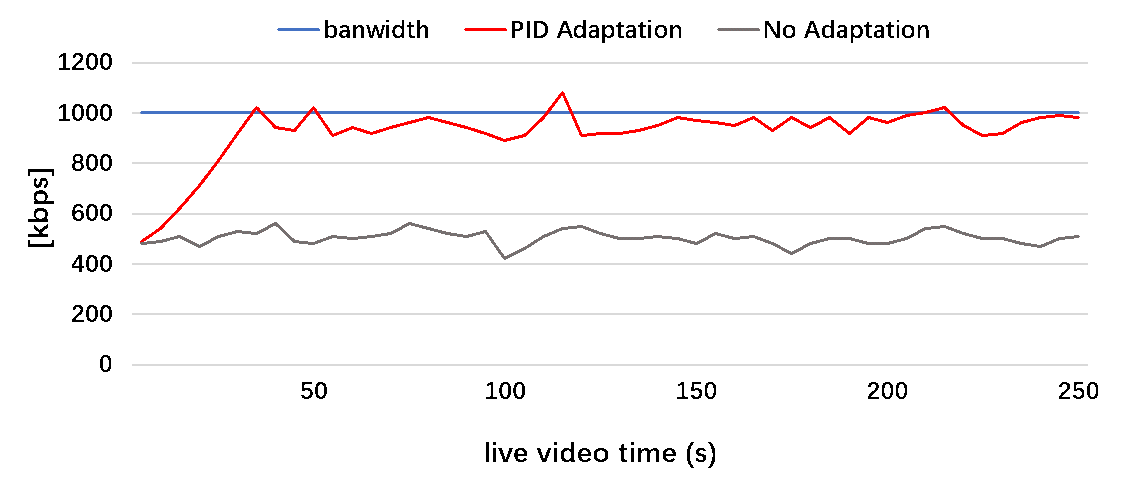
\includegraphics[width=0.6\textwidth]{clip/09-1.png}} \\
	\subfloat[长周期波动带宽的实验结果]{\label{fig:09-2}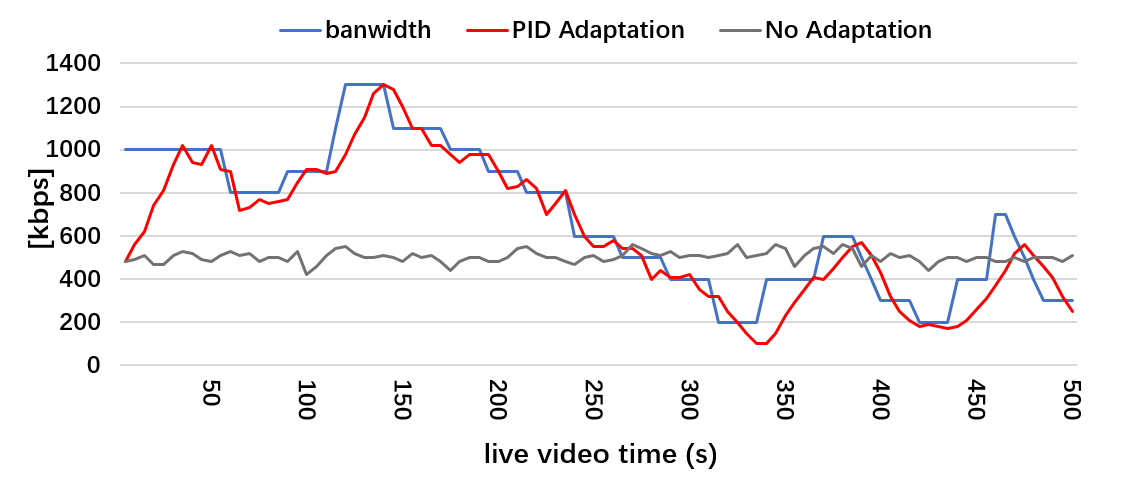
\includegraphics[width=0.6\textwidth]{clip/09-2.png}} \\
	\subfloat[短周期波动带宽的实验结果]{\label{fig:09-3}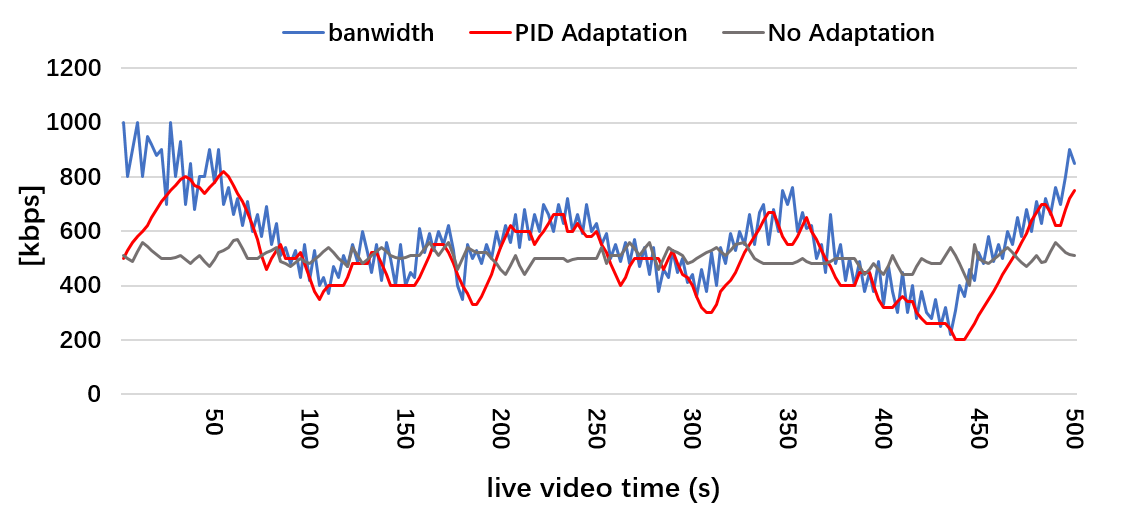
\includegraphics[width=0.6\textwidth]{clip/09-3.png}}
	\caption{直播系统在不同测试条件下码率随时间变化的情况}
	\label{fig:09}
\end{figure}

在我们的实验中,采集帧率设置为15 FPS,过程变量$\overline{S_{ASB}(t)}$的控制目标值$\tau$设为15(单位是数据段的个数,每个数据段含有一个GOP的视频),改变码率的单位为20kbps,初始码率为500kbps,对系统状态的检查周期为2秒。我们调节得到的PID控制参数$K_p$、$K_i$和$K_d$分别为0.8,0.13以及0.07。我们在3种条件下进行测试:(1)固定带宽为1Mbps;
(2)长周期波动带宽,带宽每隔40秒变化一次,在200kbps到1.4Mbps之间波动;(3)短周期波动带宽,在200kbps到1.4Mbps之间随机波动。

\subsection{结果分析}

测试结果参见图\ref{fig:09}、\ref{fig:14}和表\ref{tab:live-bandwidth}、\ref{tab:live-playtime}。

\begin{figure}[!t]
	\centering
	\subfloat[1Mbps的固定带宽的实验结果]{\label{fig:14-1}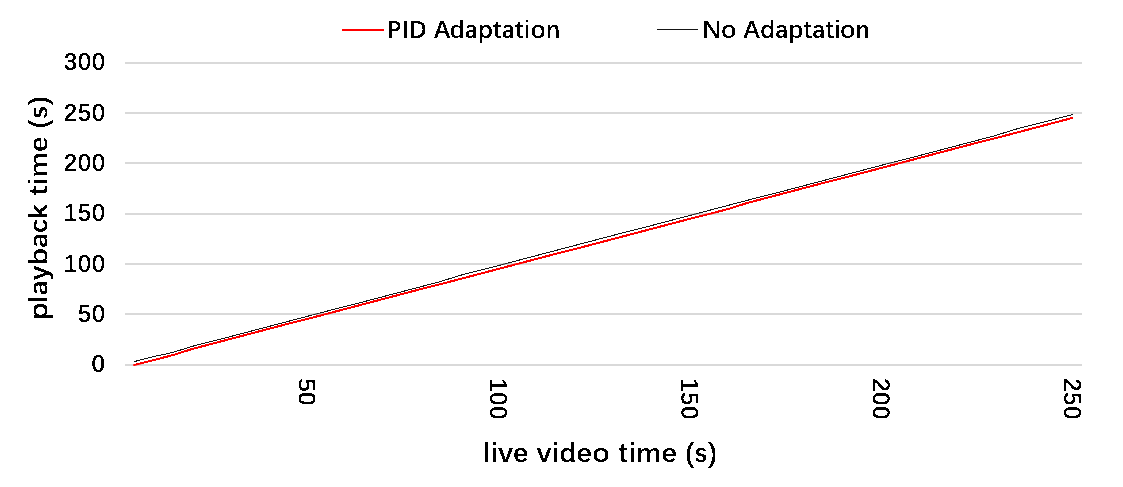
\includegraphics[width=0.65\textwidth]{clip/14-1.png}} \\
	\subfloat[长周期波动带宽的实验结果]{\label{fig:14-2}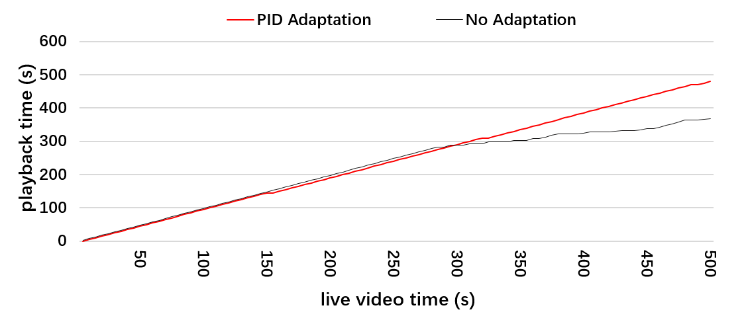
\includegraphics[width=0.65\textwidth]{clip/14-2.png}} \\
	\subfloat[短周期波动带宽的实验结果]{\label{fig:14-3}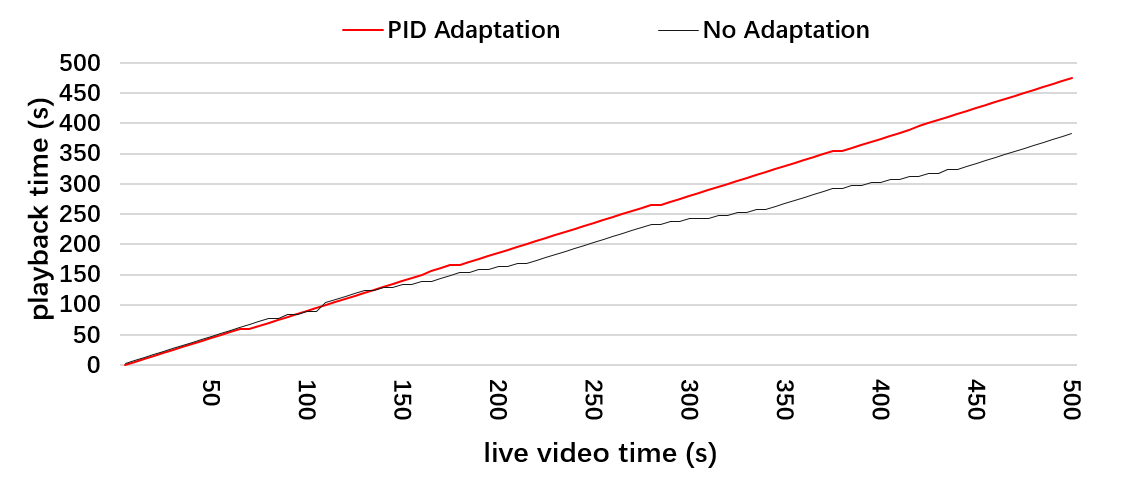
\includegraphics[width=0.65\textwidth]{clip/14-3.png}}
	\caption{直播系统在不同测试条件下播放时间占比的变化情况}
	\label{fig:14}
\end{figure}

从图\ref{fig:09-1}中可以看出,我们提出的方法使得码率在35秒以内保持上升,直到趋近带宽。从图\ref{fig:09-2}和\ref{fig:09-3}可以看出,通过我们的方法进行的调整,在一个合理的延迟以内,码率和波动的带宽基本保持同步,而且对带宽的频繁变化做了一定的平滑。如表\ref{tab:live-bandwidth}所示,我们提出的算法对于条件(1)、(2)和(3)分别将带宽占用率提高到92.1\%、88.9\%以及87.1\%。

从图\ref{fig:14-1}可以看出,对于进行调整和未进行调整的视频流,播放基本都是连续的。从图\ref{fig:14-2}和\ref{fig:14-3}可以看出,未经过调整的视频流的播放过程被频繁地中断,而经过调整的视频流的播放过程在大部分时间是连续的。如表\ref{tab:live-playtime}所示,我们所提出的方法对于条件(2)和(3)分别将播放时间占比提高到97.3\%和96.1\%,因此显著提高了播放连续性。总之,加入PID码率自适应算法比不进行码率调整的直播效果有所改善。

\begin{table*}
	\centering
	\caption{直播系统实验中的带宽利用率}
	\label{tab:live-bandwidth}
	\begin{tabular}{c|*{2}{p{1.0cm}<{\centering}|}{p{1.0cm}<{\centering}}}
		\hline\hline
		& CB & LTBV & STBV \\ \hline
		自适应调整  & 92.1\% & 88.9\% & 87.1\% \\ \hline
		不进行调整 & 50.4\% & 64.7\% & 80.3\% \\ \hline
	\end{tabular}
\end{table*}

\begin{table*}
	\centering
	\caption{直播系统实验中的播放时间占比}
	\label{tab:live-playtime}
	\begin{tabular}{c|*{2}{p{1.0cm}<{\centering}|}{p{1.0cm}<{\centering}}}
		\hline\hline
		& CB & LTBV & STBV \\ \hline
		自适应调整  & 100\% & 97.3\% & 96.1\% \\ \hline
		不进行调整 & 100\% & 73.4\% & 71.5\% \\ \hline
	\end{tabular}
\end{table*}

\section{本章小结}

本章首先对PID控制器的基本思想做了简单介绍,然后将其用到了视频流媒体中的码率自适应问题中。在选择了合适的过程变量与控制目标之后,对通用PID模型稍作修改,得到了更加直观有效的基于比例的模型,并据此给出了码率自适应算法(又称为质量控制算法)。所提出的算法相比于其他算法不仅提高了所发送视频的平均质量,还降低了质量波动,取得了更好的平滑性。当流媒体服务器把最佳视频码流传送给用户后,在下一章中我们讨论如何对视频流的解码过程进行优化,以确保尽可能多的客户端设备能达到播放高清甚至超高清视频的条件。